\subsection{Đề 2}
\Opensolutionfile{ans}[ans/ans-2-OTC4-De2]
\caulc
 \begin{ex}%[2D4N1-1]
	Cho hàm số $ f(x) $ liên tục trên khoảng $ K $ và các hằng số $ a, b, c \in K $ và $a<c<b$. Mệnh đề nào dưới đây \textbf{sai}?
	\choice
	{$ \displaystyle \int \limits^b_a f(x)  \mathrm{\,d}x = \displaystyle \int \limits^c_a f(x)   \mathrm{\,d}x + \displaystyle \int \limits^b_c f(x)   \mathrm{\,d}x $}
	{\True $ \displaystyle \int \limits^b_a  f(x) \mathrm{\,d}x \neq \displaystyle \int \limits^b_a f(t)  \mathrm{\,d}t $}
	{$ \displaystyle \int \limits^b_a k \cdot f(x)  \mathrm{\,d}x = \displaystyle k \int \limits^b_a f(x)   \mathrm{\,d}x $ với $ k \in \mathbb{R} $}
	{$ \displaystyle \int \limits^b_a  f(x) \mathrm{\,d}x = \displaystyle - \int \limits^a_b f(x)  \mathrm{\,d}x $}
	\loigiai{
		Theo tính chất của tích phân thì $ \displaystyle \int \limits^b_a  f(x) \mathrm{\,d}x = \displaystyle \int \limits^b_a f(t)  \mathrm{\,d}t $.
	}
\end{ex}

\begin{ex}%[2D4N1-3]
	Họ nguyên hàm của hàm số $f(x)=\sin x+2$ là
	\choice
	{\True $-\cos x+2x+C$}
	{$-\cos x+2x+C$}
	{$\cos x+2x+C$}
	{$\cos x+C$}
	\loigiai{
		Ta có: $\displaystyle \int f(x) dx =\displaystyle \int (\sin x+2) dx= -\cos{x}+2x+C$. \\
	}
\end{ex}

\begin{ex}%[2D4N2-2]
	Tích phân $\displaystyle\int\limits_{1}^{2} x^3\mathrm{\,d}x$ bằng
	\choice{$\dfrac{15}{3}$}{$\dfrac{17}{4}$}{$\dfrac{7}{4}$}{\True$\dfrac{15}{4}$}
	\loigiai{ 
		Ta có $\displaystyle\int\limits_{1}^{2} x^3\mathrm{\,d}x=\dfrac{x^4}{4}\Big|_1^2=\dfrac{15}{4}$.
	}
\end{ex}

\begin{ex}%[2D4N2-1]
	Nếu $\displaystyle\int\limits_1^3 f(x)\mathrm{\,d}x=2$ và $\displaystyle\int\limits_1^3 g(x)\mathrm{\,d}x=1$ thì $\displaystyle\int\limits_1^3 [3f(x)+2g(x)]\mathrm{\,d}x$ bằng
	\choice
	{$6$}
	{\True $8$}
	{$7$}
	{$5$}
	\loigiai{
		Ta có $\displaystyle\int\limits_1^3 [3f(x)+2g(x)]\mathrm{\,d}x=3\displaystyle\int\limits_1^3 f(x)\mathrm{\,d}x+2\displaystyle\int\limits_1^3 g(x)\mathrm{\,d}x=3\cdot 2+2\cdot 1=8$.
	}
\end{ex}


 \begin{ex}%[2D4H2-1]
	Cho hàm số $f\left(x\right)$ có đạo hàm trên đoạn $\left[0;2\right]$ và $f\left(0\right) = - 1$, biết $\displaystyle\int\limits_{0}^{2} f'\left(x\right)\mathrm{\,d}x = 5$. Tính $f\left(2\right)$.
	\choice
	{$f\left(2\right) = 6$}
	{$f\left(2\right) = 2$}
	{$f\left(2\right) = 5$}
	{\True $f\left(2\right) = 4$}
	\loigiai{
		\begin{center}
			$\displaystyle\int\limits_{0}^{2} f'\left(x\right)\mathrm{\,d}x = f\left(x\right) \bigg \vert_{0}^2 = f\left(2\right) - f\left(0\right) = 5 \Leftrightarrow f\left(2\right) = 4$.
		\end{center}
	}
\end{ex}
\begin{ex}%[2D4H2-1]
	Cho hàm số $f(x)$ và $F(x)$ liên tục trên $\mathbb{R}$ thoả mãn $F'(x)=f(x)$ với mọi số thực $x$. Tính   $\displaystyle \int\limits_0^1 f(x)\mathrm{\,d}x$. Biết $F(0)=2; F(1)=5$.
	\choice
	{\True $3$}
	{$4$}
	{$5$}
	{$6$}
	\loigiai{
		$\displaystyle \int\limits_0^1 f(x)\mathrm{\,d}x = F(1)-F(0)=5-2=3$.
	}
\end{ex}
\begin{ex}%[2D4H2-1]
	Tích phân $\displaystyle\int\limits_{1}^{3}\left[2f(x)+1\right]\mathrm{\,d}x=5$ thì $\displaystyle\int\limits_{1}^{3} f(x)\mathrm{\,d}x$ bằng	
	\choice
	{$3$}
	{$2$}
	{$\dfrac{3}{4}$}
	{\True$\dfrac{3}{2}$}
	\loigiai{ 
		Ta có 
			\begin{eqnarray*}
			\displaystyle\int\limits_{1}^{3} \left[2f(x)+1\right]\mathrm{\,d}x=5
			 &\Leftrightarrow&2\displaystyle\int\limits_{1}^{3} f(x)\mathrm{\,d}x+\displaystyle \int_{1}^{3} \mathrm{\,d}x =5\\
			&\Leftrightarrow& 2\displaystyle\int\limits_{1}^{3} f(x)\mathrm{\,d}x+\displaystyle 2 =5 \Leftrightarrow \displaystyle\int\limits_{1}^{3} f(x)\mathrm{\,d}x =\dfrac{3}{2}.
		\end{eqnarray*}
	}
\end{ex}

\begin{ex}%[2D4H3-3]
	Tính thể tích vật thể tạo thành khi quay hình phẳng $(H)$ quanh trục $Ox$, biết $(H)$ được giới hạn bởi các đường $y=4x^2-1$, $y=0$.
	\choice
	{\True $\dfrac{8\pi}{15}$}
	{$\dfrac{4\pi}{15}$}
	{$\dfrac{16\pi}{15}$}
	{$\dfrac{2\pi}{15}$}
	\loigiai{
		Phương trình hoành độ giao điểm $4x^2-1=0\Leftrightarrow x=\pm\dfrac{1}{2}$.\\
		Suy ra $V=\pi\displaystyle\int\limits_{-\frac{1}{2}}^{\frac{1}{2}}(4x^2-1)^2\mathrm{\,d}x=\pi\displaystyle\int\limits_{-\frac{1}{2}}^{\frac{1}{2}}(16x^4-8x^2+1)\mathrm{\,d}x=\pi\left.\left(\dfrac{16}{5}x^5-\dfrac{8}{3}x^3+x\right)\right|_{-\frac{1}{2}}^{\frac{1}{2}}=\dfrac{8\pi}{15}.$
	}
\end{ex}

 \begin{ex}%[2D4H3-1]
	Diện tích hình phẳng giới hạn bởi $2$ đường cong $y = x^2 - 2x$ và $y = 2x^2 - x - 2$ là
	\choice
	{$4$}
	{$9$}
	{$5$}
	{\True $\dfrac{9}{2}$}
	\loigiai{
		Phương trình hoành độ giao điểm $x^2 - 2x = 2x^2 - x - 2 \Leftrightarrow \hoac{& x = 1\\& x = -2.}$\\
		Vậy $\displaystyle\int\limits_{-2}^1 \left| \left(x^2 - 2x\right) - \left( 2x^2 - x - 2\right) \right|  \mathrm{\,d}x = \dfrac{9}{2}$.
	}
\end{ex}

\begin{ex}%[2D4H1-4]
	Biết $F(x)=(ax^2+bx+c)\mathrm{e}^x$ là một nguyên hàm của hàm số $f(x)=(x-1)^2\mathrm{e}^x$. Tính $S=a+2b+c$.
	\choice
	{$S=3$}
	{\True$S=-2$}
	{$S=0$}
	{$S=4$}
	\loigiai{
		Ta có $F'(x)=(ax^2+bx+c)\mathrm{e}^x+(2ax+b)\mathrm{e}^x=(ax^2+(2a+b)x+b+c)\mathrm{e}^x$.\\
		Đồng nhất hệ số với $f(x)$ ta có
		$$\heva{& a=1 \\ & 2a+b=-2\\& b+c=1}\Leftrightarrow \heva{& a=1 \\ & b=-4\\ & c=5.}$$
		Vậy $a+2b+c=-2$.
	}
\end{ex}

\begin{ex}%[2D4H3-1]
	Cho đồ thị hàm số $y=f(x)$ như hình vẽ bên dưới.
	\begin{center}
	\begin{tikzpicture}[scale=0.5, font=\footnotesize, line join=round, line cap=round, >=stealth]
		\draw[->] (-4,0)--(4,0) node[below]{$x$};
		\draw[->] (0,-1.5)--(0,4.5) node[right]{$y$};
		\node at (0,0) [below left]{$O$};
		\draw[domain=-3.2:3.5] plot(\x,{0.222*(\x)^3 - 0.222*(\x)^2 - 2*(\x) +2 });
		\draw[pattern = north east lines,opacity=.2, line width = 1.2pt,draw=none] (-3,0) plot[domain=-3:1] (\x,{0.222*(\x)^3 - 0.222*(\x)^2 - 2*(\x) +2 })--(1,0)--cycle;
		\draw[pattern = north east lines,opacity=.2, line width = 1.2pt,draw=none] (1,0) plot[domain=1:3] (\x,{0.222*(\x)^3 - 0.222*(\x)^2 - 2*(\x) +2 })--(3,0)--cycle;
		\node at (0,2) [right]{\footnotesize $2$};
		\node at (-3,0) [above left]{\footnotesize $-3$};
		\node at (1,0) [below]{\footnotesize $1$};
		\node at (3,0) [below]{\footnotesize $3$};
		\draw (0,0) circle(1pt); \draw (-3,0) circle(1pt); \draw (1,0) circle(1pt); \draw (3,0) circle(1pt); \draw (0,2) circle(1pt);
	\end{tikzpicture}
	\end{center} 
	Diện tích $S$ của hình phẳng được giới hạn bởi đồ thị hàm số $y=f(x)$ và trục $Ox$ (phần gạch sọc) được tính bởi công thức
		\choice
		{$\displaystyle S= \int \limits_{-3}^3 f(x) \, \mathrm{d}x $}
		{$\displaystyle S= \int \limits_{-3}^1 f(x) \, \mathrm{d}x + \int \limits_{1}^3 f(x) \, \mathrm{d}x $}
		{$\displaystyle S=\left| \int \limits_{-3}^3 f(x) \, \mathrm{d}x \right|$}
		{\True $\displaystyle S= \int \limits_{-3}^1 f(x) \, \mathrm{d}x - \int \limits_{1}^3 f(x) \, \mathrm{d}x $}
	\loigiai{
		Ta có diện tích cần tính bằng
		\[ S = \int \limits_{-3}^3 \left| f(x) \right| \, \mathrm{d}x = \int \limits_{-3}^1 \left| f(x) \right| \, \mathrm{d}x + \int \limits_{1}^3 \left| f(x) \right| \, \mathrm{d}x
		= \int \limits_{-3}^1 f(x)  \, \mathrm{d}x - \int \limits_{1}^3 f(x)  \, \mathrm{d}x.\]
	}
\end{ex}

\begin{ex}%[2D4V2-6]
	Tại một nhà máy, gọi $C(x)$ là tổng chi phí (tính theo triệu đồng) để sản xuất $x$ tấn sản phẩm A trong một tháng. Khi đó, đạo hàm $C'(x)$, gọi là chi phí cận biên, cho biết tốc độ tăng tổng chi phí theo lượng sản phẩm được sản xuất. Giả sử chi phí cận biên (tính theo triệu đồng trên tấn) của nhà máy được ước lượng bởi công thức
	$$
	C^{\prime}(x)=5-0,06 x+0,00072 x^2 \text { với } 0 \leq x \leq 150 .
	$$
	Biết rằng $C(0)=30$ triệu đồng, gọi là chi phí cố định. Tính tổng chi phí khi nhà máy sản xuất $100$ tấn sản phẩm A trong tháng.
	\choice
	{$570$ triệu đồng}
	{\True $470$ triệu đồng}
	{$420$ triệu đồng}
	{$440$ triệu đồng}
	\loigiai{
		Ta có:
		$$
		\begin{aligned}
			C(100)-C(0) &=\displaystyle\int\limits_0^{100} C^{\prime}(x) \mathrm{\,d} x=\displaystyle\int\limits_0^{100}\left(5-0{,}06 x+0{,}00072 x^2\right) \mathrm{\,d} x \\
			&=5 \displaystyle\int\limits_0^{100} \mathrm{\,d} x-0{,}06 \displaystyle\int\limits_0^{100} x \mathrm{\,d} x+0{,}00072 \displaystyle\int\limits_0^{100} x^2 \mathrm{\,d} x \\
			&=\left.5 x\right|_0 ^{100}-0{,}03 x^2\left.\right|_0 ^{100}+0{,}00024 x^3\left.\right|_0 ^{100}=440.
		\end{aligned}
		$$
		Suy ra $C(100)=C(0)+440=30+440=470$ (triệu đồng).\\
		Vậy khi nhà máy sản xuất $100$ tấn sản phẩm A trong tháng thì tổng chi phí là $470$ triệu đồng.
	}
\end{ex}

\Closesolutionfile{ans}
\indapan{6}{ans/ans-2-OTC4-De2}

\cauds
\Opensolutionfile{ans}[ans/ans-2-OTC4-De2-DS]
\begin{ex}%[2D4N2-2]
	Cho hàm số $f(x)=x^2$. 
	\choiceTF
	{\True $\displaystyle\int f(x)\mathrm{\,d}x=\dfrac{x^3}{3}+C$}
	{$\displaystyle\int\limits_0^2 f(x)\mathrm{\,d}x=\dfrac{7}{3}$}
	{Giả sử $F(x)$ là một nguyên hàm của $f(x)$. Khi đó $f'(x)=F(x)$}
	{\True Gọi $F(x)$ là một nguyên hàm của $f(x)$. Nếu đồ thị hàm số của $F(x)$ đi qua điểm $(3;1)$ thì $F(x)=\dfrac{x^3}{3}-8$.}
	\loigiai{
	\begin{itemchoice}
		\itemch  $\displaystyle\int x^2\mathrm{\,d}x=\dfrac{x^3}{3}+C$.\\
		\itemch $\displaystyle\int\limits_0^2 x^2\mathrm{\,d}x=\dfrac{x^3}{3}\Big|_0^2=\dfrac{8}{3}-0=\dfrac{8}{3}$.\\
		\itemch  $F(x)$ là nguyên hàm của $f(x)$ thì $F'(x)=f(x)$.\\
		\itemch Nguyên hàm $F(x)=\dfrac{x^3}{3}+C$. Mà $F(x)$ đi qua  $(3;1)$ nên $C=-8$.
	\end{itemchoice}
	}
\end{ex}
\begin{ex}%[2D4H1-1]
	Cho hàm số $f(x)$ có đạo hàm cấp một, đạo hàm cấp hai liên tục trên $\mathbb{R}$.
	\choiceTF
	{$\displaystyle\int f(x) {\,\mathrm{d}}x =f'(x)+C$}
	{\True $\displaystyle\int f'(x) {\,\mathrm{d}}x =f(x)+C$}
	{$\displaystyle\int f'(x) {\,\mathrm{d}}x =f(x)$}
	{\True $\displaystyle\int f''(x) {\,\mathrm{d}}x =f'(x)+C$}
	\loigiai
	{
		\begin{itemchoice}
		\itemch $\displaystyle\int f(x) {\,\mathrm{d}}x =f'(x)+C$ là sai theo tính chất của nguyên hàm.
		\itemch $\displaystyle\int f'(x) {\,\mathrm{d}}x =f(x)+C$ là đúng theo tính chất của nguyên hàm.
		\itemch $\displaystyle\int f'(x) {\,\mathrm{d}}x =f(x)$ sai do thiếu $C$.
		\itemch $\displaystyle\int f''(x) {\,\mathrm{d}}x =f'(x)+C$ là đúng theo tính chất của nguyên hàm.
		\end{itemchoice}
		
	}
\end{ex}
\begin{ex}%[2D4V2-6]
	Giả sử $v(t)$ là phương trình vận tốc của một vật chuyển động theo thời gian $t$ (giây), $a(t)$ là phương trình gia tốc của vật đó chuyển động theo thời gian $t$ (giây). Xét chuyển động trong khoảng thời gian từ $c$ (giây) đến $b$ (giây).
	\choiceTF
	{\True $\displaystyle\int\limits_c^b a(t)\mathrm{\,d}t=v(b)-v(c)$}
	{$\displaystyle\int\limits_c^b v(t)\mathrm{\,d}t=a(b)-a(c)$}
	{$\displaystyle\int\limits_c^b v'(t)\mathrm{\,d}t=v(c)-v(b)$}
	{\True $\displaystyle\int\limits_c^b v'(t)\mathrm{\,d}t=v(b)-v(c)$}
	\loigiai
	{
		\begin{itemchoice}
		\itemch $\displaystyle\int\limits_c^b a(t)\mathrm{\,d}t=v(b)-v(c)$ đúng do $v=a'$.
		\itemch $\displaystyle\int\limits_c^b v(t)\mathrm{\,d}t=a(b)-a(c)$ sai do $\displaystyle\int v = s+C$.
		\itemch $\displaystyle\int\limits_c^b v'(t)\mathrm{\,d}t=v(c)-v(b)$ sai do ngược cận.
		\itemch $\displaystyle\int\limits_c^b v'(t)\mathrm{\,d}t=v(b)-v(c)$ đúng do $\displaystyle\int v' = v+C$.
		\end{itemchoice}
		Là những khẳng định đúng.
	}
\end{ex}
\begin{ex}%[2D4V2-6]
Một vật chuyển động với gia tốc $a(t)=2\cos t$ (m/s$^2$).
	\choiceTF
	{\True Tại thời điểm bắt đầu chuyển động, vật có vận tốc bằng $0$. Khi đó, vận tốc của vật được biểu diễn bởi hàm số $v(t)=2\sin t$ (m/s)}
	{Vận tốc của vật tại thời điểm $t=\dfrac{\pi}{2}$ là $1$ m/s}
	{\True Quãng đường vật đi được từ thời điểm $t=0$ (s) đến thời điểm $t=\pi$ (s) là $4$ m}
	{Quãng đường vật đi được từ thời điểm $t=\dfrac{\pi}{2}$ (s) đến thời điểm $t=\dfrac{3\pi}{4}$ (s) là $2$ m}
	\loigiai{
		\begin{itemchoice}
	\itemch Ta có $v(t)=\displaystyle\int a(t) \mathrm{\,d}t=\displaystyle\int 2\cos t \mathrm{\,d}t=2\sin t+C$. \\
	Mà tại thời điểm bắt đầu chuyển động, vật có vận tốc bằng 0 nên ta có $v(0)=0$ hay $C=0$. \\
	Vậy $v(t)=2\sin t$.
\itemch Vận tốc của vật tại thời điểm $t=\dfrac{\pi}{2}$ là $v\left(\dfrac{\pi}{2}\right)=2\sin \dfrac{\pi}{2}=2$ (m/s).
\itemch Quãng đường vật đi được từ thời điểm $t=0$ (s) đến thời điểm $t=\pi$ (s) là
		$$
		\displaystyle\int_0^\pi v(t) \mathrm{\,d}t=\displaystyle\int_0^\pi 2 \sin t \mathrm{\,d}t=-\left.2 \cos t\right|_0 ^\pi=-2 \cos \pi-(-2 \cos 0)=4\,(\mathrm{m}).
		$$
	\itemch  Quãng đường vật đi được từ thời điểm $t=\dfrac{\pi}{2}$ (s) đến thời điểm $t=\dfrac{3\pi}{4}$ (s) là
		$\displaystyle\int_{\frac{\pi}{2}}^{\frac{3 \pi}{4}} v(t) \mathrm{\,d}t
		=\displaystyle\int_{\frac{\pi}{2}}^{\frac{3 \pi}{4}} 2 \sin t \mathrm{\,d}t
		=-2 \cos t\Big| _{\frac{\pi}{2}} ^{\frac{3 \pi}{4}}
		=-2 \cos \dfrac{3\pi}{4}-\left(-2 \cos \dfrac{\pi}{2}\right)
		=\sqrt{2}\,(\mathrm{m}).$
	\end{itemchoice}
		}
\end{ex}
\Closesolutionfile{ans}
\indapan{2}{ans/ans-2-OTC4-De2-DS}

\Opensolutionfile{ans}[ans/ans-2-OTC4-De2-KQ]
\caukq

\begin{ex}%[2D4C3-1]
	\immini{Cho hàm số bậc ba $y=f(x)$ có đồ thị là đường cong trong hình bên. Biết hàm số $f(x)$ đạt cực trị tại hai điểm $x_1$, $x_2$ thỏa mãn $x_2=x_1+2$ và $f\left(x_1\right)+f\left(x_2\right)=0$. Gọi $S_1$ và $S_2$ là diện tích của hai hình phẳng được gạch trong hình bên. Tỉ số $\dfrac{S_1}{S_2}$ bằng}{
		\begin{tikzpicture}[scale=1, font=\footnotesize, line join=round, line cap=round,>=stealth]
			\def \xmin{-0.7};
			\def \xmax{4.5};
			\def \ymin{-2.5};
			\def \ymax{2.7};
			\draw[->] (\xmin, 0.) -- (\xmax,0.) node[anchor=north] {$x$};
			\draw[->] (0.,\ymin) -- (0.,\ymax) node[anchor=west] {$y$};
			\clip(\xmin+0.1,\ymin+0.1) rectangle (\xmax-0.1,\ymax-0.1);
			\fill[pattern=north east lines,opacity=0.4] (0,0) plot[smooth,domain=2:1] (\x,{(\x-2)^3-3*(\x-2)})--(1,0)--cycle;
			\fill[pattern=north west lines,opacity=0.4] (0,0) plot[smooth,domain=1:2] (\x,{(\x-2)^3-3*(\x-2)})--(2,2)--cycle;
			\draw[dashed] 
			(1,0) node[below]{$x_{1}$}|-(1,2)--(2,2)
			(3,0)node[below left]{$x_{2}$}--(3,-2)
			;
			\draw[smooth] plot[domain=\xmin:\xmax] (\x,{(\x-2)^3-3*(\x-2)});
			\draw 
			(2,\ymin)--(2,\ymax)
			(1.4,.5) node{$S_{2}$}
			(1.75,1.5) node{$S_{1}$}
			;
			\draw[fill=black] (0,0) circle (1pt) node[below left] {$O$};
	\end{tikzpicture}}
\shortans{$0{,}6$}
	\loigiai
	{Giả sử $f(x)=ax^3+bx^2+cx+d$ với $a\neq 0$.\\
		Từ đồ thị ta có $\lim\limits_{x\to +\infty}f(x)=+\infty\Rightarrow a>0$.\\
		Ta có $f'(x)=3ax^2+2bx+c$. Vì $x_1$, $x_2$ là hai điểm cực trị của $f(x)$ nên $$f'(x)=3a(x-x_1)(x-x_2)=3a(x-x_1)(x-x_1-2)=3a(x-x_1)^2-6a(x-x_2).$$
		Suy ra $f(x)=\displaystyle\int f'(x) \mathrm{\,d}x=a(x-x_1)^3-3a(x-x_1)^2+C$.\\
		Từ hình vẽ ta có $f(x_1+1)=0$ nên $a-3a+C=0\Leftrightarrow C=2a$.\\
		Do đó $f(x)=a(x-x_1)^3-3a(x-x_1)^2+2a\Rightarrow f(x_1)=2a$.\\
		Diện tích của hình chữ nhật (hai hình phẳng được gạch) là $S_1+S_2=1\cdot f(x_1)=2a$.\\
		Mặt khác,
		\begin{eqnarray*}
			S_2&=&\displaystyle\int\limits_{x_1}^{x_1+1} f(x)  \mathrm{\,d}x= \int\limits_{x_1}^{x_1+1} \left[a(x-x_1)^3-3a(x-x_1)^2+2a\right]  \mathrm{\,d}x\\
			&=& \left[\dfrac{a(x-x_1)^4}{4}-a(x-x_1)^3+2ax\right]\Bigg|_{x_1}^{x_1+1}\\
			&=& \left(\dfrac{a}{4}-a+2ax_1+2a\right)-2ax_1\\
			&=& \dfrac{5a}{4}.
		\end{eqnarray*}
		Suy ra $S_1=2a-S_2=2a-\dfrac{5a}{4}=\dfrac{3a}{4}$.\\
		Vậy $\dfrac{S_1}{S_2}=\dfrac{3}{5}$.
	}
\end{ex}


\begin{ex}%[2D4H1-4]
	Gọi  $ F(x)$ là một nguyên hàm của hàm số $ f(x)=\dfrac{\mathrm{e}^{2 x}-6}{\mathrm{e}^x}$,  biết $ F(0)=7$. Tính tổng các nghiệm của
	phương trình  $ F(x)=5$ (làm tròn đến hàng phần trăm).
	\shortans{$1{,}79$}
	\loigiai{
		Ta có $F(x)=\displaystyle \int \dfrac{\mathrm{e}^{2x}-6}{\mathrm{e}^x} \mathrm{d} x
		=  \displaystyle \int \left( \mathrm{e}^x -6 \mathrm{e}^{-x} \right) \mathrm{d} x
		=\mathrm{e}^x+6 \mathrm{e}^{-x}   + C.$\\
		Với $F(0)=7 \Leftrightarrow  1+6+C=7 \Leftrightarrow C=0$. Suy ta $F(x)=\mathrm{e}^{x}+6\mathrm{e}^{-x}$.\\
		Xét 
		\begin{eqnarray*}
			F(x)=5
			&\Leftrightarrow & \mathrm{e}^x+6 \mathrm{e}^{-x}   + 0=5\\
			&\Leftrightarrow & \mathrm{e}^{2x}-5 \mathrm{e}^x+6=0\\
			&\Leftrightarrow & \hoac{ \mathrm{e}^x=2  \\ \mathrm{e}^x =3} \Leftrightarrow  \hoac{ x=\ln 2  \\ x=\ln 3.}
		\end{eqnarray*}
		Vậy tổng các nghiệm là $\ln 2+ \ln 3 = \ln 6 \approx 1{,}79$.
	}
\end{ex}

\begin{ex}%[2D4H3-3]
	Xét vật thể $(\mathcal{T})$ nằm giữa hai mặt phẳng $x=-1$ và $x=1$. Biết rằng thiết diện của vật thể cắt bởi mặt phẳng vuông góc với trục $Ox$ tại điểm có hoành độ $x$ $(-1\leq x\leq 1)$ là một hình vuông có cạnh $2\sqrt{1-x^2}$. Tính thể tích vật thể $(\mathcal{T})$ (làm tròn đến hàng phần trăm).
	\shortans{$5{,}33$}
	\loigiai{
		Diện tích thiết diện là $S(x)=4(1-x^2)$.\\
		Suy ra thể tích vật thể $(\mathcal{T})$ là $V=\displaystyle \int \limits_{-1}^1 4(1-x^2) \mathrm{\,d}x=\left( 4x-\dfrac{4x^3}{3}\right) \Bigg|_{-1}^1=\dfrac{16}{3}\approx 5{,}33$.
	}
\end{ex}

\begin{ex}%[2D4V2-6]
	Một vật chuyển động với gia tốc được cho bởi hàm số $a(t)=5\cos t$ (m/s$^2$). Lúc bắt đầu chuyển động vật có vận tốc $2{,}5$ m/s. Tính gia tốc của vật (đơn vị m/s$^2$) tại thời điểm vận tốc đạt giá trị lớn nhất trong $\pi$ (s) đầu tiên.
	\shortans{$0$}
	\loigiai{
		Vận tốc của vật được biểu diễn bởi hàm số $v(t)=\displaystyle\int a(t) \mathrm{\,d}t=\displaystyle\int 5\cos t \mathrm{\,d}t=5\sin t+C$.\\
		Khi bắt đầu chuyển động, vật có vận tốc $2{,}5$ m/s nên ta có
		$$
		v(0)=2{,}5 \Leftrightarrow 5 \sin 0+C=2{,}5 \Leftrightarrow C=2{,}5
		$$
		Suy ra $v(t)=5\sin t+2{,}5$. \\
		Ta có $\sin t \le 1 \Rightarrow 5\sin t+2{,}5\leq 7{,}5$. \\
		Vận tốc đạt giá trị lớn nhất khi $\sin t=1 \Rightarrow t=\dfrac{\pi}{2}$. \\
		Khi đó, gia tốc của vật tại thời điểm $t=\dfrac{\pi}{2}$ là $a\left(\dfrac{\pi}{2}\right)=5\cos \left(\dfrac{\pi}{2}\right)=0$ m/s$^2$}
\end{ex}

\begin{ex}%[2D4C3-1]
	Cho parabol $( P )\colon y=x^2$ và hai điểm $A$, $B$ thuộc $( P )$ sao cho $AB=2$. Tìm giá trị lớn nhất của diện tích hình phẳng giới hạn bởi parabol $( P )$ và đường thẳng $AB$ (Làm tròn đến hàng phần trăm).
	\shortans{$1{,}33$}
	\loigiai{ 
\begin{center}
		\begin{tikzpicture}[line join=round, line cap = round, >=stealth, scale=.8,font=\footnotesize,transform shape]
		\draw[line width=0.5pt,gray!50] ; % Hiển thị lưới đồ thị.
		\draw[->] (-3,0)--(3,0) node[below]{\footnotesize $x$};
		\draw[->] (0,-2)--(0,5) node[right]{\footnotesize $y$};
		\clip (-3,-2) rectangle (3,4.5);
		\draw (0,0) node[below left]{\footnotesize $O$};
		%\draw (0,0) node[below right]{\footnotesize $O$};
		%\draw (-\d/\c-\m,\a/\c)--(-\d/\c+\m,\a/\c) (-\d/\c,\a/\c-\m)--(-\d/\c,\a/\c+\m);
		\draw[samples=500, ] plot (\x,{(\x)^2});
		\node[below] at (-1,4) {$y=x^2$};
		\node[below] at (1,0) {$1$};
		\path
		(-1,1) coordinate (A)
		(1.5,2.25) coordinate (B)
		;
		\draw[-] (A)--(B);
		\foreach \x/\g in {A/-135,B/-45}
		\fill[black] (\x) circle(1pt) ($(\x)+(\g:3mm)$) node{$\x$};
		\fill[pattern=north east lines]plot[domain=-1:1.5](\x,{(\x)^2})--plot[domain=1.5:-1](\x,{1/2*(\x)+3/2})--cycle;
	\end{tikzpicture}
\end{center}
			Gọi $A( a;a^2 )$ và $B( b;b^2 )$ là hai điểm thuộc $( P )$ sao cho $AB=2$.\\
			Không mất tính tổng quát giả sử $a<b$.\\
			Theo giả thiết ta có $AB=2$ nên
			$$( b-a )^2+( b^2-a^2 )^2=4\Leftrightarrow ( b-a )^2[ ( b+a )^2+1 ]=4.$$
			Do $( b+a )^2+1\ge 1$ nên $(b-a)^2 \le 4$ hay $|b-a|\ge 2$.\\
			Phương trình đường thẳng đi qua hai điểm $A$ và $B$ là $y=( b+a )x-ab$.\\
			Gọi $S$ là diện tích hình phẳng giới hạn bởi parabol $( P )$ và đường thẳng $AB$ ta có\\ \indent
			$S=\displaystyle \int\limits_{a}^{b}{[ ( a+b )x-ab-x^2 ] \mathrm{\, d}x}
			=\left [ ( a+b )\dfrac{x^2}{2}-abx-\dfrac{x^3}{3} \right] \bigg|_{a}^{b}
			=\dfrac{{{( b-a )}^3}}{6}$.\\
			Mặt khác $|b-a|\ge 2$ nên $ S=\dfrac{( b-a )^3}{6}\le \dfrac{2^3}{6}$. \\
			Vậy $S_{\max }=\dfrac{4}{3}$, dấu bằng xảy ra khi và chỉ khi $a=-b=\pm 1$.
	}
\end{ex}

\begin{ex}%[2D4V3-2]
	\immini{Bạn An cần mua một chiếc gương có viền là đường parabol bậc $2$ (xem hình vẽ). Biết rằng đoạn $AB=60$ cm, $OH=30$ cm. Diện tích của chiếc gương bạn An mua bằng bao nhiêu cm$^2$?
	\shortans{$1200$}
	}{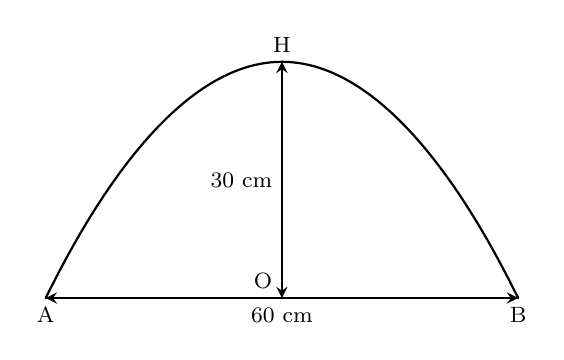
\begin{tikzpicture}[scale=1,font=\footnotesize,line join = round, line cap = round, >= stealth]
			%\tkzDefPoints{0/0/A, 5/0/x, 1.5/1/y, 0/5/z}
			\draw[thick] (-3,0) parabola bend (0,3) (3,0);
			\draw[thick,<->] (-3,0)--(3,0);
			\draw[thick,<->] (0,0)--(0,3);
			\draw (0,3) node[above]{H} (-3,0) node[below]{A} (3,0) node[below]{B} (0,0) node[above left]{O};
			\draw (0,0) node[below]{$60$ cm};
			\draw[](0,1.5) node[left]{$30$ cm};
			%\clip (-3.5,-1) rectangle (3.5,3.5);
	\end{tikzpicture}}
	\loigiai{
		\immini{Xét hệ trục tọa độ $Oxy$, sao cho gốc $O$ trùng với điểm $O$, trục $Ox$ trùng với tia $OB$, trục $Oy$ trùng với tia $OH$.\\
			Khi đó $B(30;0)$, $H(0;30)$.\\
			Phương trình Parabol đi qua $A$, $H$, $B$ có dạng\\ $y=ax^2+b\quad(P)$.
		}{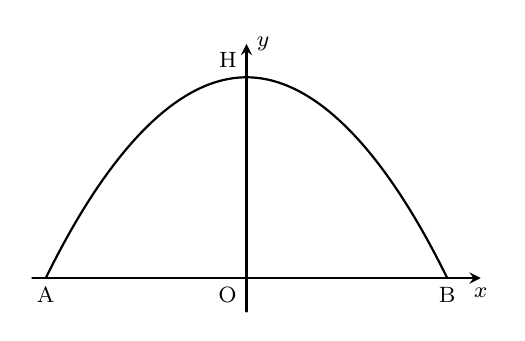
\begin{tikzpicture}[scale=.85,font=\footnotesize,line join = round, line cap = round, >= stealth]
				%\tkzDefPoints{0/0/A, 5/0/x, 1.5/1/y, 0/5/z}
				\draw[thick] (-3,0) parabola bend (0,3) (3,0);
				\draw[thick,->] (-3.2,0)--(3.5,0) node[below]{$x$};
				\draw[thick,->] (0,-0.5)--(0,3.5) node[right]{$y$} ;
				\draw (0,3) node[above left]{H} (-3,0) node[below]{A} (3,0) node[below]{B} (0,0) node[below left]{O};
				%\draw (0,0) node[below]{$60$ cm};
				%\draw[](0,1.5) node[left]{$30$ cm};
				%\clip (-3.5,-1) rectangle (3.5,3.5);
		\end{tikzpicture}}
		\noindent $H\in (P)\Rightarrow 30=b.\quad(1)$\\
		$B\in (P)\Rightarrow 0=a\cdot 30^2+30\Rightarrow a =-\dfrac{1}{30}.\quad(2)$\\
		Từ $(1)$, $(2)\Rightarrow (P)\colon y=-\dfrac{1}{30}x^2+30$.\\
		Diện tích của chiếc gương là
		\[\displaystyle\int\limits_{-30}^{30}\left(-\dfrac{1}{30}x^2+30\right)\mathrm{\,d}x=\left.\left(-\dfrac{x^3}{90}+30x\right)\right|_{-30}^{30}=1200\, \text{(cm$^2$)}.\]
	}
\end{ex}
\Closesolutionfile{ans}
\indapan{6}{ans/ans-2-OTC4-De2-KQ}